When we observe an animal grappling with the decision to either explore or exploit, we often imagine this decision is based on reward. For example, if a bee goes in a familiar direction \textit{to gather nectar}, it is said to be exploiting past knowledge for environmental reward. If it goes in an unfamiliar direction \textit{to gather nectar}, it is said to be exploring for reward. Because the environment is partly unkown to the bee, it cannot rationally choose which action it should be doing, exploiting or exploring \textit{to gain more reward}. It is this uncertainty \textit{about returning the most rewards} that makes explore-exploit choices a dilemma. It is also this uncertainty which ensures there is no tractable mathematical solution for explore-exploit questions about reward \citep{Thrun1992a,Dayan1996,Ishii2002,Simsek2006,Gershman2018b}. We illustrate this view in Fig. \ref{fig:bee}a.

The choice between exploring and exploiting is indeed faced routinely by learners of all kinds, including foraging bees, business organizations, humans, worms, monkeys, rodents, birds, children, and computer algorithms \citep{Gupta2006,Sutton2018,Woodgate2017,Lee2011a,Schulz2018a,Calhoun2014,Wang2019,Sumner2019,Auersperg2015}. But is reward really fundamental to it? Because in the natural world exploration already finds two explanations. If there is no reason to expect a reward, exploration is described theoretically as a search for information, what we will call curiosity \citep{Berlyne1950,Schmidhuber1991,Kidd2015,deAbril2018,Jaegle2019,Friston2016}. On the other hand, if reward is expected, then exploration gets re-interpreted as we described above, as a search for reward, and this specific interpretation is what leads the famous dilemma \citep{Kelly1956,Berger-Tal2014,Dayan1996,Thrun1992,Mehlhorn2015,Kobayashi2019}. 

Our goal is to maximize the return of reward in this paper, but have come to argue curiosity is better goal for exploration in this problem. Our ``curiosity trick'' to the dilemma is a counterintuitive suggestion, but we will prove exploration is better handled by a curiosity search even when the long-term goal is rewards. We illustrate our view of dilemma, and our trick, in Fig. \ref{fig:bee}b.

\begin{figure}
	\begin{fullwidth}
	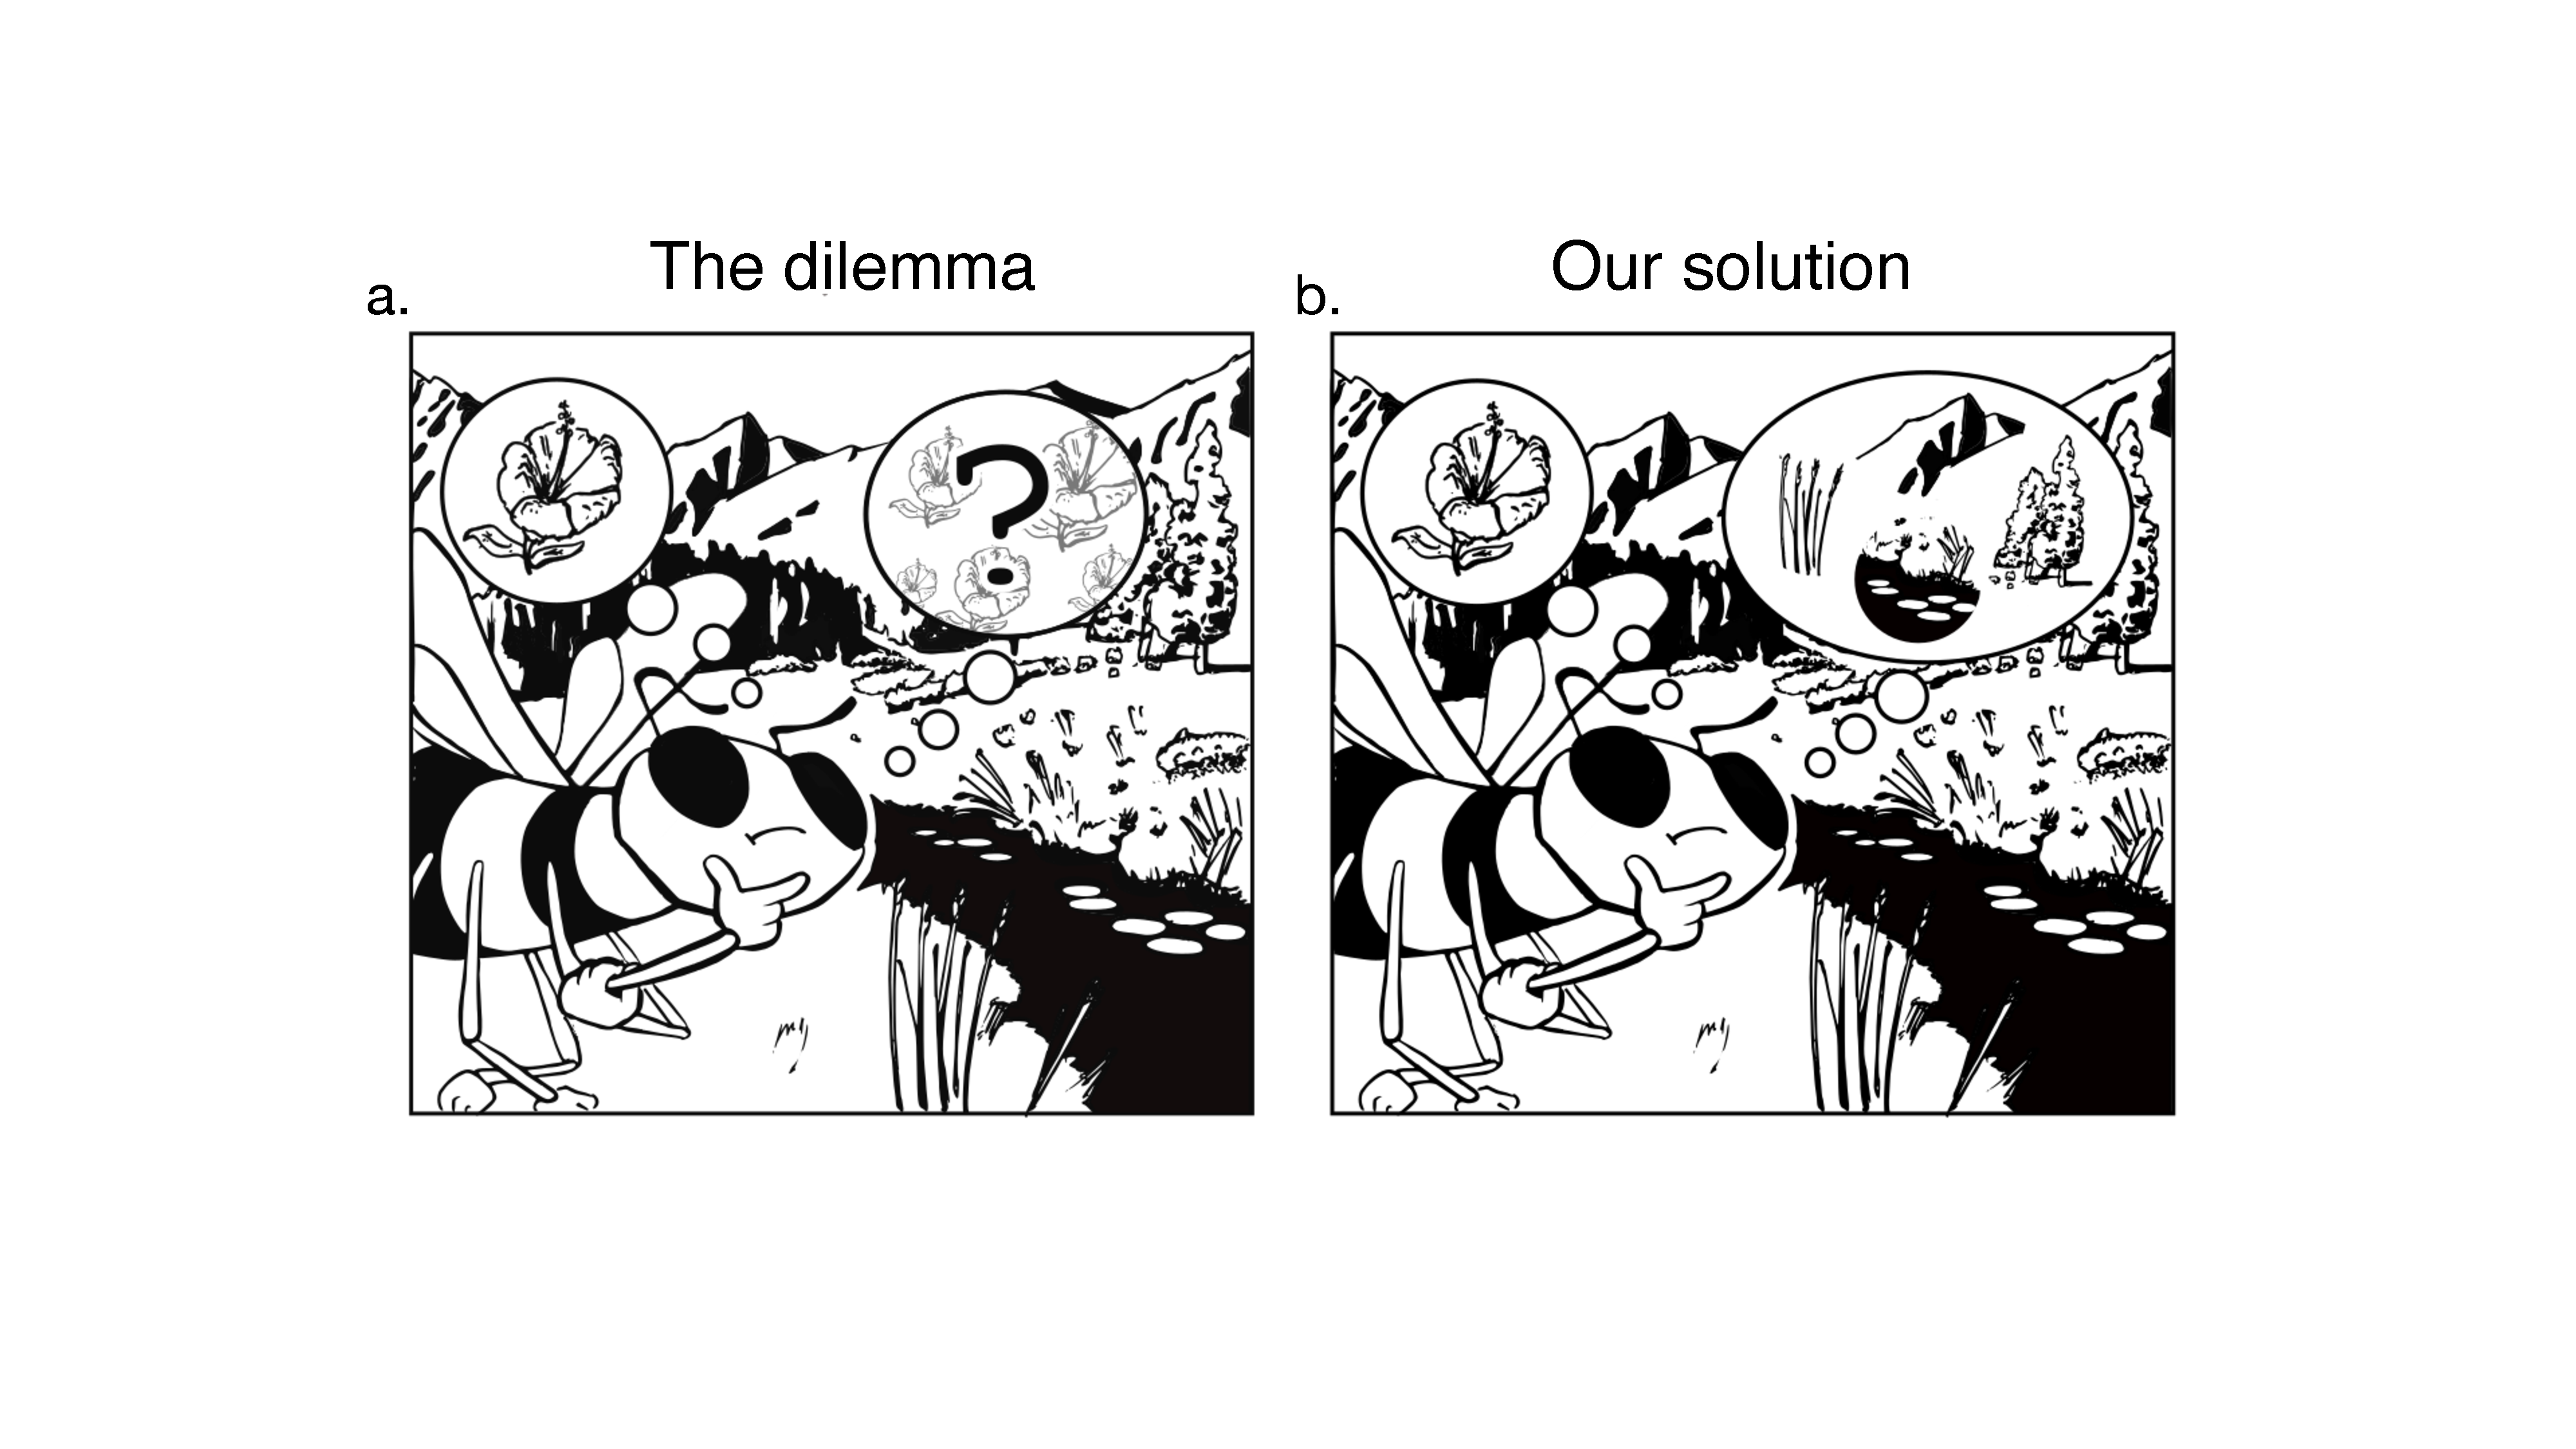
\includegraphics[width=.55\linewidth]{dilemma-draft-elife/img/bee.pdf} 
	\caption{Two views of exploration and exploitation. \textbf{a}. The classic dilemma: either exploit an action with a known reward (e.g., return to the previous flower) or explore other actions on the chance they will return a better outcome. The central challenge here is that the outcome of exploration is uncertain, and filled with questions. \textbf{b}. An alternative view of the dilemma, with two goals: either maximize rewards \textit{or} maximize information value with a curious search of the environment. \textit{Artist credit}: Richard Grant.}
	\label{fig:bee} 
	\end{fullwidth}
\end{figure}

The first half of this paper is devoted to developing a view of curiosity that is mathmatically general. This effort, it turns out, lets us make a new contribution to information theory--defining subjective information value without considering meaning at all. This lets us also develop new proofs that define an ideal curious search. The second half uses these first results to prove curiosity can generate an optimal value solution to all explore-exploit decisions that are normally based on rewards.
